\section{Methodology}
\label{sec:method}

The following subsections provide insights on the methodology one followed 
in order to achieve the objectives listed in Section~\ref{sec:objectives}.

\subsection{Solution Representation and Evaluation Function for the CVRP}
\label{subsec:spec-enti}

All strategies and algorithms proposed in Section~\ref{sec:intro} to tackle 
the CVRP were implemented in C\slash C++, following descriptions distributed 
over several sources~\cite{Toth2002, Michalewicz2004, Thangiahl1996, 
Psaraftis1983391, Osman1993}. 
The following sub-sections provide some details about each 
implementation.\vertbreak

\subsubsection{Solution Representation}
\label{subsubsec:sol-rep}

Regarding general data structures for representing important entities and 
quantities used in the CVRP, the following are of particular importance:

\begin{itemize}

    \item \verb?Station?: Represents a demand point which should be visited by 
            a vehicle. An instance of \verb?Station? has information about (1) the 
            demand point's index (as given in the dataset), (2) demand point's 
            $(x,y)$ coordinates, (3) the demand value of the point, (4) the 
            route it (currently) belongs to and (5) pointers to the previous and 
            next demand points in the route it belongs to.
    \item \verb?Route?: Represents a single vehicle's route. Contains 
            information about (1) an identifying index for the route, (2) the 
            current cost (i.e. length) of the route, (3) the 
            current amount of goods supplied 
            by the route, (4) the number of demand points currently in the 
            route and (5) pointers to the first and last \verb?Station? in the 
            route.
\end{itemize}\vertbreak

The entities listed above are important for the solution representations used in 
this problem. Since solutions in the CVRP are usually represented as sequences 
of demand points closed by the depot (i.e. routes), in this case 
we treat a solution $S$ as set of linked lists of \verb?Station? instances:
\[ depot \rightarrow station[i] \rightarrow station[k] \rightarrow station[l] \rightarrow ... \rightarrow depot \] 

Each 
linked list is described by an associated \verb?Route? instance. A special 
aggregating data structure \verb?CVRP? is used to represent a graph for the 
CVRP, i.e. in practice a \verb+CVRP+ instance is our solution representation 
$S$. This entity holds a list of \verb?Route? instances, each one 
containing several \verb?Station? instances, linked between each other 
according to their order within a route.\vertbreak

\subsubsection{Evaluation Function}
\label{subsubsec:eval-fun}

The CVRP aims at minimizing the total distance traveled by the different 
vehicles when following their respective routes. Therefore, we use the total 
distance between \verb+Station+ instances within a \verb+Route+, for all the 
\verb+Route+ instances in a solution $S$, as the evaluation function 
$e(S)$. Given a \verb+Route+ $r$, we sometimes use $e(r)$ for referring to 
the distance traveled by a vehicle within that single route.\vertbreak

\subsection{Clarke and Wright Savings (CWS) Algorithm}
\label{subsec:overview}

After the initial literature review phase, documented in
 Section~\ref{sec:intro}, the Clarke and Wright Savings (CWS) algortithm, as 
presented in Section 5.2.1 in~\cite{Toth2002}, was identified as an appropriate 
heuristic for tackling CVRP. It presents itself as a clearly constructive 
heuristic, due to its principle of building `complex' routes by merging more 
simple routes --- initially in the form $(0, i, 0)$ --- via links $(i,j)$, 
associated with a special quantity designated by `savings'.\vertbreak

The CWS presents two versions, (1) a parallel version and (2) a sequential 
version, further explained in Section~\ref{subsec:cws-p}.

\subsection{Construction of the Savings List}
\label{subsec:savings}

One of the key features of the CWS algorithm is the use of the `saving' 
entities, already discussed in previous sections. In addition to general data 
structures for representing a CVRP problem (described in 
Section~\ref{subsec:spec-enti}), the 
CWS algorithm implementation defines the representation of a saving quantity, 
\verb?Saving?, which contains information about (1) the indexes of demand 
points $(i,j)$ (i.e. instances of \verb?Station?) to which the saving is 
associated and (2) the actual saving value.\vertbreak

The description provided 
in~\cite{Toth2002} suggests the calculation of every $s_{ij}$ for all 
$i, j = 1, ..., n$, only imposing $i \neq j$ as a constraint. For $N$ nodes, 
this would result in a list of size $N(N - 1)$. This number can be further 
reduced by realizing the following:

\begin{itemize}

    \item The savings associated with the depot can be discarded, which 
            reduces the size by a parcel of $2(N - 1)$.
    \item $s_{ij} = s_{ji}$, which reduces the size of the list to half. This 
            translates into a reduction of memory usage, however, requires an 
            extra computation on the \verb?merge? routines, as mentioned in 
            Section~\ref{subsec:cws-p}.

\end{itemize}\vertbreak

Taking the considerations above into account, we get a final size for the 
savings list of $\frac{1}{2}((N - 1)(N - 2))$. This is easy to imagine in 
matrix form, as seen in~\ref{eq:savings}. Imagine a $N \times N$ matrix, with 
the rows and columns as the node indexes $i$ and $j$, so that each cell is a 
$(i,j)$ combination. The elements marked by an \textbf{x} are those which are 
eliminated by the simplifications mentioned above, while those marked with 
\textbf{o} are kept. This is important in computational terms, since both 
parallel and sequential versions of the CWS algorithm cycle through the entire 
savings list, with the possibility of repetitions for the sequential 
case.\vertbreak

\begin{equation}
\begin{bmatrix} \textbf{x} & \textbf{x} & \textbf{x} & \textbf{x} \\ 
                \textbf{x} & \textbf{x} & \textbf{o} & \textbf{o} \\ 
                \textbf{x} & \textbf{x} & \textbf{x} & \textbf{o} \\ 
                \textbf{x} & \textbf{x} & \textbf{x} & \textbf{x} \\ \end{bmatrix}
    \label{eq:savings}
\end{equation}\vertbreak

In addition, Step 1 of the CWS algorithm indicates that the savings list should 
be ordered in descending order of magnitude. To do so, we use a custom 
implementation of the Quicksort 
algorithm~\cite{Hoare:1961:AP:366622.366642}.

\subsection{Versions of the CWS}
\label{subsec:cws-p}

As denoted in Section~\ref{subsec:savings}, the simplifications performed while 
constructing the savings list have implications on the \verb?merge? routines, 
for both versions, specifically the evaluation of the conditions shown 
below:\vertbreak

\begin{algorithmic}[1]
\If {($i + 1$ is depot) $\wedge$ ($j - 1$ is depot)}

    \State Join route $r_k$ (containing $i$) and route $r_l$ (cont. $j$), via 
    \Statex[2] the link $(i,j)$
    

\ElsIf {($i - 1$ is depot) $\wedge$ ($j + 1$ is depot)} 
    \State Join route $r_k$ (containing $i$) and route $r_l$ (cont. $j$), via 
    \Statex[2] the link $(j,i)$
\Else 
    \State At least one of $(i,j)$ is interior to a route $r_k$ or $r_l$. 
    \Statex[2] Abort.
\EndIf
\end{algorithmic}\vertbreak

In short, the conditions shown above compensate the elimination of the symmetric 
pairs of points $(i,j)$ and $(j,i)$, by evaluating a merge between two routes 
via the link $(j,i)$ if trying it via the link $(i,j)$ does not work.\vertbreak

In addition to the conditions given above, the procedures taken upon the 
establishment of a link between two previously unconnected routes is similar 
among the two versions. Specifically, considering route $r_l$ is merged to route 
$r_k$ (i.e. route $r_l$ ceases to exist) all \verb?Station? entities previously 
part of a route $r_l$ are updated to belong to route $r_k$, the pointers of the 
linking \verb?Station? entities are updated (as these no longer point to the 
depot) and the information held by the \verb?Route? entity of route $r_l$ is 
appropriately merged with that of route $r_k$.\vertbreak

The parallel and sequential version of the CWS algorithm mostly differ in the 
way the various route merging operations are applied, not on the nature of 
the single merge operation. For the parallel version, the algorithm cycles 
through the savings list once, performing merges between several routes 
along the way, i.e. it does not `stick' to merging other routes to a particular 
route, given a pair of points $(i,j)$ it attempts to merge any two routes that 
include the edges $i$ and $j$.\vertbreak

For the sequential version, the algorithm `sticks' to a route $r_k$, cycles 
through the savings list and evaluates if a link $(i,j)$ is suitable for 
merging a route $r_l$ with $r_k$ (i.e. only links $(i,j)$ in which either $i$ 
or $j$ are in the edges of $r_k$ are considered suitable). If that is the case, 
that link $(i,j)$ is discarded from the list, and the algorithm returns to the 
top of the savings list, since the new merging operation may have enabled a 
previous pair $(i,j)$. This is repeated until the algorithm reaches the end of 
the savings list. In its turn, the whole procedure is repeated for each 
remaining route in the algorithm's route list\cprotect\footnote{In our case, 
the process 
is only applied to a new route in the list if the associated \verb?Route? 
entity is active.}.

\subsection{Constraints in CWS Route Mergings}
\label{subsec:const}

Whenever a merge operation between two routes $r_i$ and $r_j$ is attempted --- in 
both the parallel and sequential cases --- the implemented version of the CWS 
algorithm takes the following evaluations into account (let $c(r)$ represent 
the quantity of goods delivered within a route $r$):

\begin{itemize}

    \item Total amount of goods supplied by the two routes must be less than 
            a vehicle's capacity $C$, i.e. $c(r_i) + c(r_j) \le C$. If 
            such a condition is not verified, the merge operations is not allowed.
    \item Demand points on a link $(i,j)$, associated with a saving quantity $s_{ij}$ 
            under consideration for a route merge, must not be interior to 
            a route.
    \item Demand points on a link $(i,j)$, associated with a saving quantity $s_{ij}$ 
            under consideration for a route merge, must not belong to the same 
            route.

\end{itemize}

If the previously listed conditions are met, the merge operation is allowed to 
go ahead, the \verb?Station? $(i,j)$ instances, at the appropriate edges of each 
route $r_i$ and $r_j$, are linked in order to form a new route. The value of the 
new route, $e(r_n)$ is calculated according to 
$e(r_n) = e(r_i) + e(r_j) - s_{ij}$.\vertbreak

Although no constraints related to the number 
of routes are imposed in the \verb?merge? functions, the CWS algorithm always 
determines the optimal number of routes for the sequential version, while it 
sometimes reports a sub-optimal number for the parallel 
version, as verified in the results given in Section~\ref{sec:results}.

\subsection{2-Opt Local Search Heuristic}
\label{subsec:2-opt}

Given the results of the constructive heuristic obtained after a run of the CWS 
algorithm, we run a 2-opt local search heuristic over the results of each route 
$R_i$. This procedure is based on that described in~\cite{Psaraftis1983391, 
Thangiahl1996}. Its objective is to remove crossings of links in a route, while 
preserving the orientation of the routes, which reduces the distance of the 
route (see Section 6.2 in~\cite{Michalewicz2004}).\vertbreak

In this case, we try to find a better solution $R'_i$, i.e. one for which the 
evaluation function $d(R'_i) < d(R_i)$, within the neighborhood of $R_i$, i.e. 
the routes one can reach by swapping two nodes in $R_i$.\vertbreak

The 2-opt local search routine was implemented according to the specification 
given below, which shows an exchange between all combination of nodes at 
positions $k$ and $m$, within all routes calculated by the CWS algorithm, 
$R$ (let $R[k]$ and $R[m]$ represent the \verb+Station+ instances at indexes 
$k$ and $m$ within a \verb+Route+ $R$, and $d(R[k], R[m])$ represent the 
euclidean distance between stations $R[k]$ and $R[m]$):\vertbreak

\begin{algorithmic}[1]
\ForAll{final CWS routes $R$} 

    \State best\_distance $ \leftarrow d(R_i)$ 

    \For{ ($k \leftarrow 1$; $k <$ size($R_i$) $- 1$; $k$++)} 

        \For{ ($m \leftarrow (m + 1)$; $m <$ size($R_i$); $m$++)} 

            \State new\_distance $ \leftarrow $
            \Statex[4] $d(R_i)$ 
            \Statex[4] + $d(R_i[k - 1], R_i[m])$ 
            \Statex[4] + $d(R_i[k], R_i[m + 1])$ 
            \Statex[4] - $d(R_i[k - 1], R_i[k])$ 
            \Statex[4] - $d(R_i[m], R_i[m + 1])$

            \If {new\_distance $ < $ best\_distance}

                \State best\_distance $ \leftarrow $ new\_distance
                \State swap($R_i[k],R_i[m]$)
            \EndIf

        \EndFor

    \EndFor

\EndFor
\end{algorithmic}\vertbreak

After an initial evaluation of the potential gains of an exchange between 
nodes $k$ and $m$, if a lower cost $d(R'_i) < d(R_i)$ is detected, the 
actual \verb?swap()? procedure is applied. Given a route arrangement, such as 
the one shown in Figure~\ref{fig:2-opt-before}, the \verb?swap(W,Y)? procedure 
changes it into Figure~\ref{fig:2-opt-after}.

%\[ depot \rightarrow r[i] \rightarrow r[a] \rightarrow r[b] \rightarrow r[j] \rightarrow depot \] 
%\[ depot \rightarrow r[j] \rightarrow r[b] \rightarrow r[a] \rightarrow r[i] \rightarrow depot \] 

\begin{figure}[h!]
    \centering

    \subfigure[]{
        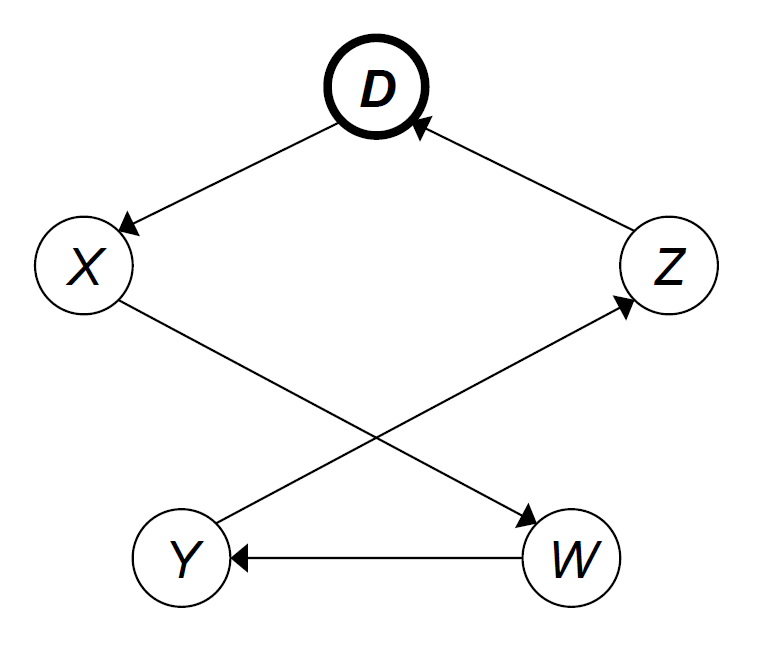
\includegraphics[width=0.25\textwidth] {figures/2-opt-before.png}
        \label{fig:2-opt-before}
    }

    \subfigure[]{
        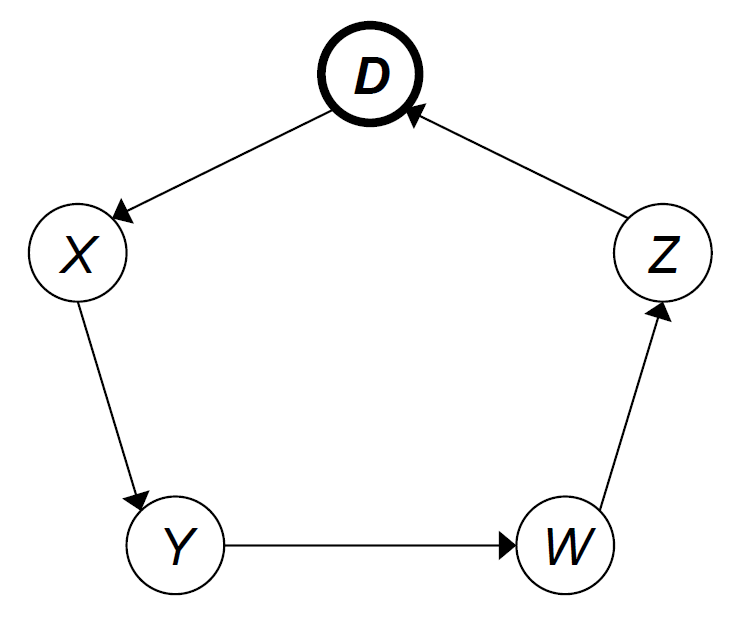
\includegraphics[width=0.25\textwidth] {figures/2-opt-after.png}
        \label{fig:2-opt-after}
    }

    \cprotect\caption{Graphical depiction of the \verb?swap()? procedure, 
        in this case between nodes $W$ and $Y$ of a given route composed by 
        four nodes ($D$ represents a depot).}
    \label{fig:2-opt}

\end{figure}

\subsection{Simulated Annealing (SA)}
\label{subsec:sa}

The version of the Simulated Annealing (SA) algorithm implemented here follows 
the specification given in Section~\ref{subsec:metaheuristics}. Its main 
`deviations' from other versions of the algorithm are (1) the mechanism for 
neighborhood generation (details in Section~\ref{subsec:1-ichange}) and (2) the 
method for setting an initial temperature $T_s$ (see 
Section~\ref{subsec:cooling}).\vertbreak

The SA algorithm was implemented in a separate C\slash C++ module which uses 
the basic CVRP data structures given in Section~\ref{subsec:spec-enti} and uses 
the CWS module to generate initial solutions. As a result of this 
implementation, a new heuristic --- 1-interchange local search (see 
Section~\ref{subsec:1-ichange} --- was added to the basic CVRP module.

\subsection{1-Interchange Local Search Heuristic}
\label{subsec:1-ichange}

The neighborhood generation mechanism used in line 9 of the SA algorithm 
described in Section~\ref{subsec:metaheuristics} is based on 
a $\lambda$-interchange method introduced by 
I. Osman~\cite{Osman1993,Thangiahl1996,Toth2002}. Regarding the work presented 
here, the 
adoption of such heuristic represents an evolution compared to the 
simpler 2-opt local search heuristic described in Section~\ref{subsec:2-opt}: 
now, instead of restricting the interchanges between two stations $s_i$ and 
$s_j$ to a single route $r$, a neighbor $S_n$ of a solution $S$ is 
generated by inserting\slash exchanging one station into\slash between 
different routes $r_i$ and $r_j$. Such 1-interchange mechanism includes two 
different operations:

\begin{itemize}

    \item \textbf{(0,1) or (1,0):} Extracting a station $s_i$ from a route 
        $r_i$ and inserting it in a route $r_j$.
    \item \textbf{(1,1):} Swapping stations $s_i$ and $s_j$ between their 
        initial routes $r_i$ and $r_j$.

\end{itemize}\vertbreak

In order to remove crossings of links in the routes $r_i$ and $r_j$ --- which 
may happen due to the re-configuration caused by the 1-interchange 
procedure --- the same 2-opt local search method described in 
Section~\ref{subsec:2-opt} is applied to both routes at the end of the `core' 
1-interchange process.\vertbreak

\subsection{Initial Temperature Calculation}
\label{subsec:cooling}

The results of SA algorithms depend on the tuning of multiple parameters: (1) 
initial temperature $T_s$, (2) cooling ratio $\alpha$, (3) termination 
condition and (4) halting criterion. We follow a method for determining $T_s$ 
which is similar to that used in the hybrid Tabu Search - Simulated 
Annealing algorithm proposed by I. Osman in~\cite{Osman1993}.\vertbreak

We define the acceptance probability of a new solution $S_n$ (derived from a 
current solution 
$S_c$ via a 1-interchange procedure) as (see line 16 of the algorithm defined 
in Section~\ref{subsec:metaheuristics}):

\begin{equation*}
    P(S_n) = \left\{ 
        \begin{array}{rl}
            e^\frac{-(e(S_n) - e(S_c))}{T_c} &\mbox{ \text{if $e(S_n) \geq e(S_c)$}} \\
            1 &\mbox{ \text{if $e(S_n) < e(S_c)$}}
        \end{array} \right.
    \label{eq:sa-accept}
\end{equation*}

where $e(.)$ is the evaluation function and $T_c$ is the current temperature. 
Considering an initial solution $S_i$, we determine the initial temperature 
$T_s$ by calculating $T$ for which $P(\text{min}(\Delta_e)) = 0.5$, 
where $\Delta_e = e(S_n) - e(S_i)$.\vertbreak

Given an initial solution $S_i$, its entire neighborhood obtained via a 
1-interchange local search heuristic is analyzed and the changes in the 
evaluation function $\Delta_e$ 
are recorded for each feasible interchange\footnote{I.e. all changes that 
result in routes not exceeding the vehicle capacity constraint.}. We then 
apply the following expression to determine $T_s$:

\[T_s = \frac{\text{min}(\Delta_{e})}{\text{ln}(0.5)}\]

\subsection{Genetic Algorithm (GA)}
\label{subsec:ga}

The version of the Genetic Algorithm (GA) algorithm implemented in this work 
follows the specifications given in Section~\ref{subsubsec:gen-al}. Its main 
specificities are (1) the mechanism for 
population selection (see Section~\ref{subsec:random-tournament}); (2) the 
crossover method for generating new solutions (see 
Section~\ref{subsec:cross-over}); (3) the mutation process applied to 
new solutions generated by the crossover process (see 
Section~\ref{subsec:mutations}).\vertbreak

As with previous cases, the GA algorithm was implemented in a separate 
C\slash C++ module which uses the basic CVRP data structures described in 
Section~\ref{subsec:spec-enti}. The following input 
parameters must be given to our GA implementation:

\begin{itemize}
    \item Solutions provided by the CWS (both parallel and sequential) and SA 
            algorithms.
    \item Number of generations to produce $G$.
    \item Population size $N$.
    \item Mutation probability for the crossover process $M \in [0.0, 1.0]$
\end{itemize}\vertbreak

In our case, we include the solutions provided 
by the parallel and sequential versions of the CWS algorithm, along with that 
provided via SA, in the initial population $P(t_0)$. The remaining $N - 3$ 
elements of the initial population $P(t_0)$ are randomly generated, taking into 
account the capacity $C$ and route number $R$ constraints implicit in the CWS and 
SA solutions.

\subsection{Random Tournament Selection}
\label{subsec:random-tournament}

The population selection strategy used in our GA instance (step 6 on the listing 
shown in Section~\ref{subsubsec:gen-al}) is based on simple 
Random Tournament Selection, with a sample size of two, i.e. one pair of 
solutions $(S_1,S_2)$ is picked at random from $P(t - 1)$ and one chooses that 
$S_n$ with lowest evaluation function value $e(S_n)$. In addition, our strategy 
automatically elects the best 10\% of $P(t - 1)$ to $P'(t)$, the set of `fittest' 
solutions (those with lower values of $e(.)$), which are excused from 
participating in the tournament.\vertbreak 

The process is summarized in pseudo-code in the following listing ($N$ is the 
population size, given as argument to the algorithm):\vertbreak

\begin{algorithmic}[1]

\State sort $P(t - 1)$
\State add top 10\% of $P(t - 1)$ to $P'(t)$, 
\Statex[1] exclude them from $P(t - 1)$

\While{size of $P'(t) < \frac{N}{2}$}

    \Repeat
        \State select random pair $(S_1,S_2)$ from $P(t - 1)$
    \Until{$S_1 != S_2$}

    \If {$e(S_1) \le e(S_2)$}

        \State add $S_1$ to $P'(t)$, exclude it from $P(t - 1)$

    \ElsIf {$e(S_1) > e(S_2)$}

        \State add $S_2$ to $P'(t)$, exclude it from $P(t - 1)$

    \EndIf

\EndWhile

\end{algorithmic}\vertbreak

\subsection{Crossover Approach}
\label{subsec:cross-over}

Partial-Mapped Crossover (PMX) and Order Crossover (OX)~\cite{Toth2002} are 
examples of crossover operators, specially devised for the Traveling Salesman 
Problem (TSP). Besides the special characteristics imposed by the TSP to 
crossover operations, the CVRP adds 
additional constraints, specifically the division of a 
typical TSP tour in several routes $R$ and capacity of routes $C$. As proposed 
by~\cite{Toth2002} in Section 6.5.3, we tackle the multiple route constraint by 
extending the CVRP into a TSP-like representation, with multiple copies of the 
depot in-between routes. E.g. for a CVRP with 8 stations and 3 routes (with 
$D$ representing the depot) such as

\[ D \rightarrow 1 \rightarrow 5 \rightarrow 8 \rightarrow D \] 
\[ D \rightarrow 3 \rightarrow 2 \rightarrow D \] 
\[ D \rightarrow 7 \rightarrow 6 \rightarrow 4 \rightarrow D \] 

one would get the following TSP-like representation:

\[ D \rightarrow 1 \rightarrow 5 \rightarrow 8 \rightarrow D \rightarrow 3 \rightarrow 2 \rightarrow D \rightarrow 7 \rightarrow 6 \rightarrow 4 \rightarrow D \] 

In addition, we apply a PMX-based crossover operation similar to the Best 
Route Better Adjustment (BRBAX) recombination mechanism presented 
in~\cite{Bermudez2010}. The following listing summarizes the offspring 
generation procedure (which includes the BRBAX-based crossover operation) in 
pseudo-code (let $C$ be the capacity constraint of the CVRP under consideration; 
$Q_r$ be the quantity of goods supplied in a route $r$; $R$ the number of 
routes of the solutions contained in the set $P'(t)$; $D$ represents the depot):\vertbreak

\begin{algorithmic}[1]

\While{size of $O(t) < \frac{N}{2}$}

    \Repeat
        \State select random pair $(P_1,P_2)$ from $P'(t)$
    \Until{$P_1 != P_2$}

    \State initialize `offspring' solution $S_o$

    \State sort routes of $P_1$ according to $C - Q_r$, 
    \Statex[2] in ascending order
    \State add best $\frac{R}{2}$ routes of $P_1$ to $S_o$

    \ForAll{routes $r$ in $P_2$} 
        \ForAll{stations $s$ in route $r_i$} 
            \If {$s_i$ not in $S_o$}
                \State add $s_i$ to $S_o$, in order, 
                \Statex[5] with $D$ delimiting routes of $P_2$
            \EndIf
        \EndFor
    \EndFor

    \If {number of routes in $S_o > R$}
        \State condense $S_o$ into $R$ routes
    \EndIf

    \If {CVRP constraints are met by $S_o$}
        \State add $S_o$ to $O(t)$
    \Else
        \State discard $S_o$
    \EndIf

\EndWhile

\end{algorithmic}\vertbreak

While the route condensation method is not described here, it is partially commented 
in the method \verb+FromTSPRepresentation()+, in file \verb+Evolutionary.cpp+.\vertbreak

\subsection{Mutations}
\label{subsec:mutations}

The `offspring' solutions of the set $O(t)$, generated via the crossover 
process described in Section~\ref{subsec:random-tournament}, can be slightly 
altered by a mutation procedure which occurs with probability 
$M \in [0.0, 1.0]$, defined as an input parameter.\vertbreak 

The mutation process is 
simple, consisting in the application of two simple heuristics, already 
applied in the previous CWS and SA implementations: 

\begin{itemize}
    \item A 1-interchange procedure (see Section~\ref{subsec:1-ichange}) between two random routes of a solution 
        $S_o \in O(t)$.
    \item A 2-opt local search method (see Section~\ref{subsec:2-opt}) on a random route 
        of a solution $S_o \in O(t)$.
\end{itemize}


